\documentclass[10pt, aspectratio=169]{beamer}

\usepackage{hyperref}
\hypersetup{
    colorlinks=false,
    % linkcolor=umBlue,
    % filecolor=magenta,
    % urlcolor=cyan,
    % pdftitle={Overleaf Example},
    % pdfpagemode=FullScreen,
    }
\usepackage{xcolor}
\usepackage{amsmath}
\usepackage{wrapfig}
\usepackage{graphicx}
\usepackage{helvet}
\usepackage[T1]{fontenc}
\usepackage{tikz}
\usetikzlibrary{shapes, arrows, calc, positioning, patterns}
\usetikzlibrary{decorations.pathreplacing}
\usepackage{amsmath,amssymb, amsfonts}
\usepackage{lipsum}
\usepackage{datetime}
\usepackage{setspace}
\usepackage{listings}
\usepackage{fancyvrb}
%%% Local Variables:
%%% mode: latex
%%% TeX-master: "../main"
%%% End:

\renewcommand{\familydefault}{\sfdefault}
\renewcommand\mathfamilydefault{}
\newcommand{\colorbf}[1]{{\color{umGreen}\textbf{#1}}}

\newdateformat{dmydate}{%
  \twodigit{\THEDAY}~\monthname[\THEMONTH] \THEYEAR%
}

%%%%%%%%%%%%%%%%%%%%%%%%%%%%%%%%%%%%
%% eqauation
%%
\DeclareMathAlphabet{\mathbfsf}{\encodingdefault}{\sfdefault}{bx}{n}
% \renewcommand{\vec}[1]{\mathbfsf{#1}}
\newcommand{\vect}[1]{\vec{\mathbf{#1}}}
\newcommand{\brak}[1]{\langle{#1}\rangle}
\newcommand{\rbrak}[1]{\left({#1}\right)}
\newcommand{\sbrak}[1]{\left[{#1}\right]}
\newcommand{\cbrak}[1]{\left\{{#1}\right\}}
\newcommand{\abrak}[1]{\left|{#1}\right|}
\newcommand{\intInf}{\int_{-\infty}^{+\infty}}
\newcommand{\intinf}{\int_{-\infty}^{\infty}}
\newcommand{\conj}{\mathlarger{*}}%
\newcommand{\Psiconj}{\Psi^\conj}
\newcommand{\Psixt}{\Psi\rbrak{x,t}}
\newcommand{\hi}{\hat{i}}
\newcommand{\hj}{\hat{j}}
\newcommand{\hk}{\hat{k}}
\newcommand{\hx}{\hat{i}}
\newcommand{\hy}{\hat{j}}
\newcommand{\hz}{\hat{k}}
\newcommand{\vB}{\vect{B}}
\newcommand{\vE}{\vect{E}}
\newcommand{\vD}{\vect{D}}
\newcommand{\vH}{\vect{H}}
\newcommand{\curl}[1]{\vect{\nabla}\times\vect{#1}}
\newcommand{\divg}[1]{\vect{\nabla}\cdot\vect{#1}}

% quote
\newcommand{\q}[1]{``#1''}

%%% Local Variables:
%%% mode: latex
%%% TeX-master: "../main"
%%% End:


%%% Local Variables:
%%% mode: latex
%%% TeX-master: "../main"
%%% End:


\mode<presentation>{%
    \usetheme{fqs}
    \usecolortheme{fqs}
}

\title[UM Template]{A Beamer Theme for State University of Malang}
\subtitle[YABT]{This is a Beamer Theme Styled After State University of Malang's (UM) Powerpoint Template.}
\titlebackground{fqsstyle/assets/gambar-um.jpg}
\author{Firman Q. S.} % Your name
\institute[Universitas Negeri Malang] % Your institution as it will appear on the bottom of every slide, may be shorthand to save space
{\noindent
    \textit{firman.qashdus.2103216@students.um.ac.id}\par% Your email address
    Physics Departement\par
    Students\par
}
\date{\dmydate\today} % Can be changed to a custom date

\setbeamersize{text margin left=.05\pdfpagewidth,text margin right=.05\pdfpagewidth}

\begin{document}
%%%%%%%%%%%%%%%%%%%%%%%%%%%%%%%%%%%%
%% TITLE PAGE: with background image
%%
\maketitle

%%%%%%%%%%%%%%%%%%%%%%%%%%%%%%%%%%%%
%%  TITLE PAGE: without background image
%%
{
  \setbeamertemplate{headline}{}
  \begin{frame}
      %%%%%%%%%%%%%%%%%%%%%%
      %% Featured Image (comment or delete if not used)
      %%
      \begin{tikzpicture}[overlay, remember picture]
          \node[left=1.0cm] at (current page.1){%
              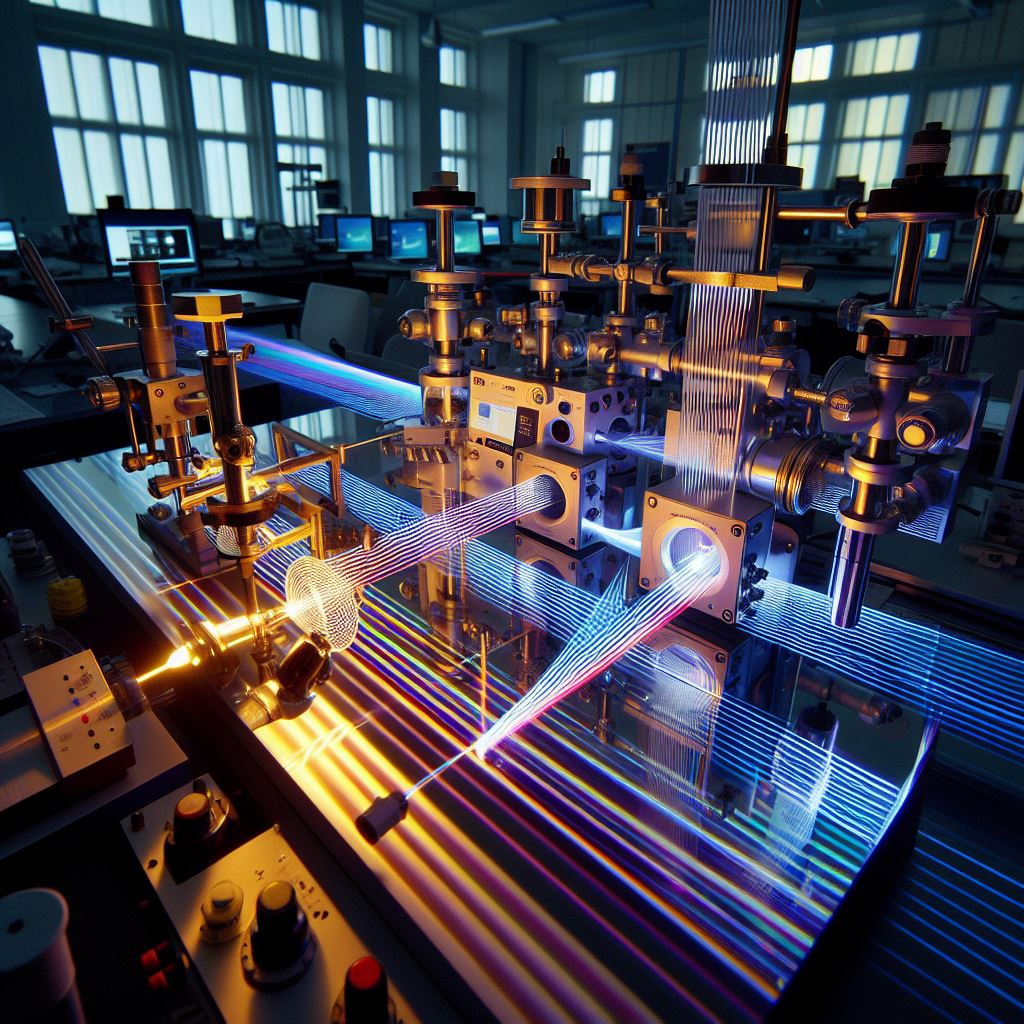
\includegraphics[width=6.5cm]{contents/images/optics-lab}
          };
      \end{tikzpicture}
      % the title page itself
      \titlepage%
  \end{frame}
}

%%%%%%%%%%%%%%%%%%%%%%%%%%%%%%%%%%%%
%% SECTION PAGE: without background image
%%
\section{Installation}
{
    \setbeamertemplate{headline}{}
    \begin{frame}
        \sectionpage%
        %%%%%%%%%%%%%%%%%%%%%%
        %% Featured Image
        %%
        \begin{tikzpicture}[overlay,remember picture]
            \node[left=2cm] at (current page.2){%
                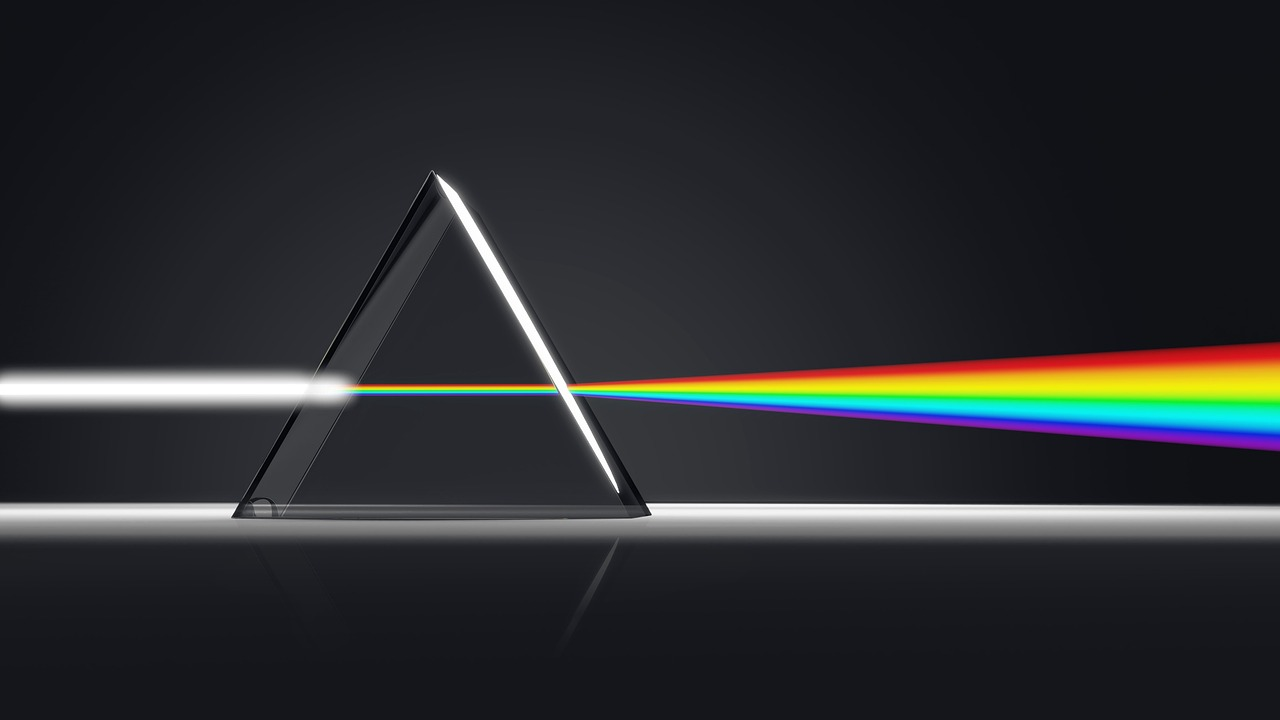
\includegraphics[width=6.5cm]{contents/images/prism-light-dispersion}
            };
        \end{tikzpicture}
    \end{frame}
}

\begin{frame}{How to Use?}
    To use this latex beamer template in local machine you need to do the following:
    \begin{enumerate}
        \item Install latex distibution
              \begin{itemize}
                  \item[$\blacktriangleright$] for \textbf{Linux}: \href{https://www.google.com/search?q=how to install latex in linux?}{TeX Live}
                  \item[$\blacktriangleright$] for \textbf{Mac}: \href{https://www.google.com/search?q=how to install mac tex on mac?}{Mac Tex}
                  \item[$\blacktriangleright$] for \textbf{Windows}: \href{https://www.google.com/search?q=how to install miktex in windows?}{MiKTeX}
              \end{itemize}
        \item Install \LaTeX editor, The following is a list of common editors that you can use
              \begin{itemize}
                  \item[$\blacktriangleright$] \href{https://code.visualstudio.com/}{Visual Studio Code} with \href{https://marketplace.visualstudio.com/items?itemName=James-Yu.latex-workshop}{LaTex Workshop} extension.
                  \item[$\blacktriangleright$] \href{http://www.xm1math.net/texmaker/}{Texmaker}.
                  \item[$\blacktriangleright$] \href{http://texstudio.org/}{TeXStudio}.
                  \item[$\blacktriangleright$] \href{https://www.gnu.org/software/emacs/}{GNU Emacs} with its \href{https://gnu.org/software/auctex/}{AUC-TeX} Package.
               \end{itemize}
        \item Download 3 this beamer template and compile.
    \end{enumerate}
\end{frame}

%%%%%%%%%%%%%%%%%%%%%%%%%%%%%%%%%%%%
%% SECTION PAGE: without background image
%%
\section{List}
{
    \setbeamertemplate{headline}{}
    \begin{frame}
        \sectionpage%
        %%%%%%%%%%%%%%%%%%%%%%
        %% Featured Image
        %%
        \begin{tikzpicture}[overlay,remember picture]
            \node[left=2cm] at (current page.2){%
                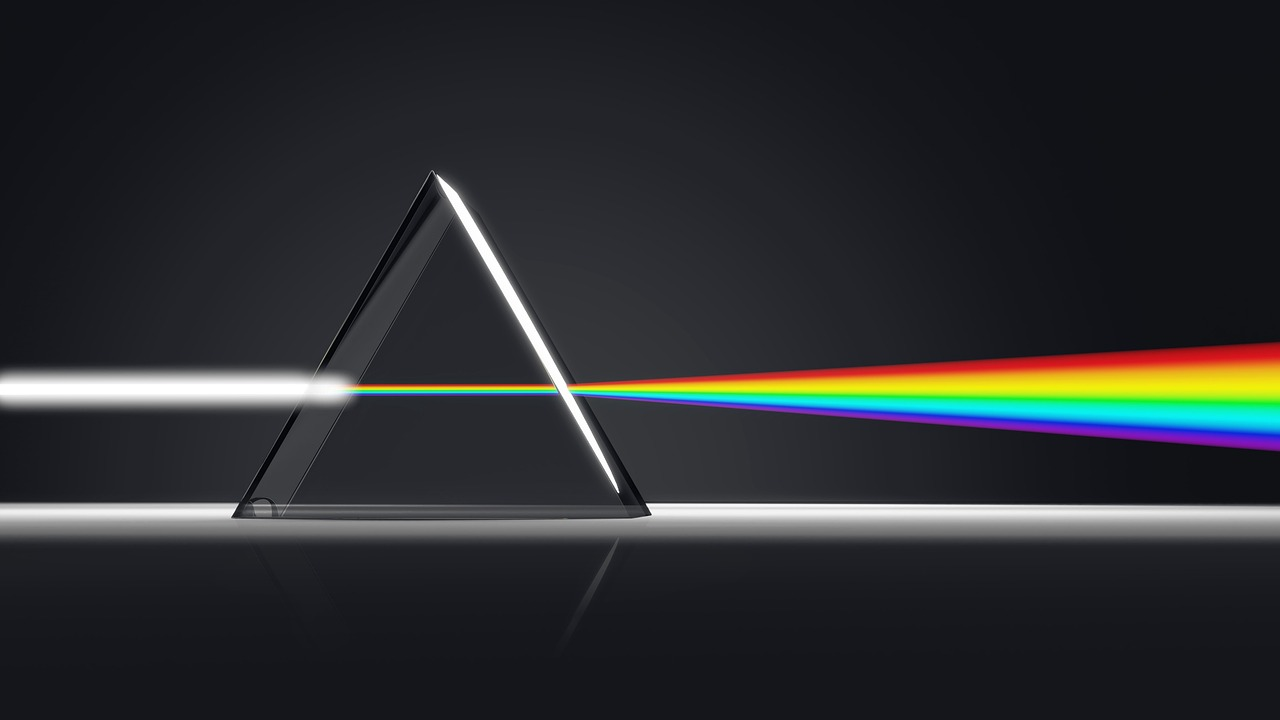
\includegraphics[width=6.5cm]{contents/images/prism-light-dispersion}
            };
        \end{tikzpicture}
    \end{frame}
}

\begin{frame}{Title}
    \begin{itemize}
    \item \lipsum[1][5]
        \begin{itemize}
        \item \lipsum[1][5]
            \begin{itemize}
            \item \lipsum[1][5]
            \end{itemize}
        \end{itemize}
    \end{itemize}

    \begin{block}{Block Title}
        Consider a \colorbf{function} $\rho(r,\phi)$ such that
        \begin{equation*}
            R_{\mu \nu} - {1 \over 2}R \, g_{\mu \nu} + \Lambda g_{\mu \nu}= {8 \pi G \over c^4} T_{\mu \nu}
        \end{equation*}
    \end{block}
\end{frame}

%%%%%%%%%%%%%%%%%%%%%%%%%%%%%%%%%%%%
%% SECTION PAGE: without background image
%%
\section{Multiple Columns}
{
    \setbeamertemplate{headline}{}
    \begin{frame}
        \sectionpage%
        %%%%%%%%%%%%%%%%%%%%%%
        %% Featured Image
        %%
        \begin{tikzpicture}[overlay,remember picture]
            \node[left=2cm] at (current page.2){%
                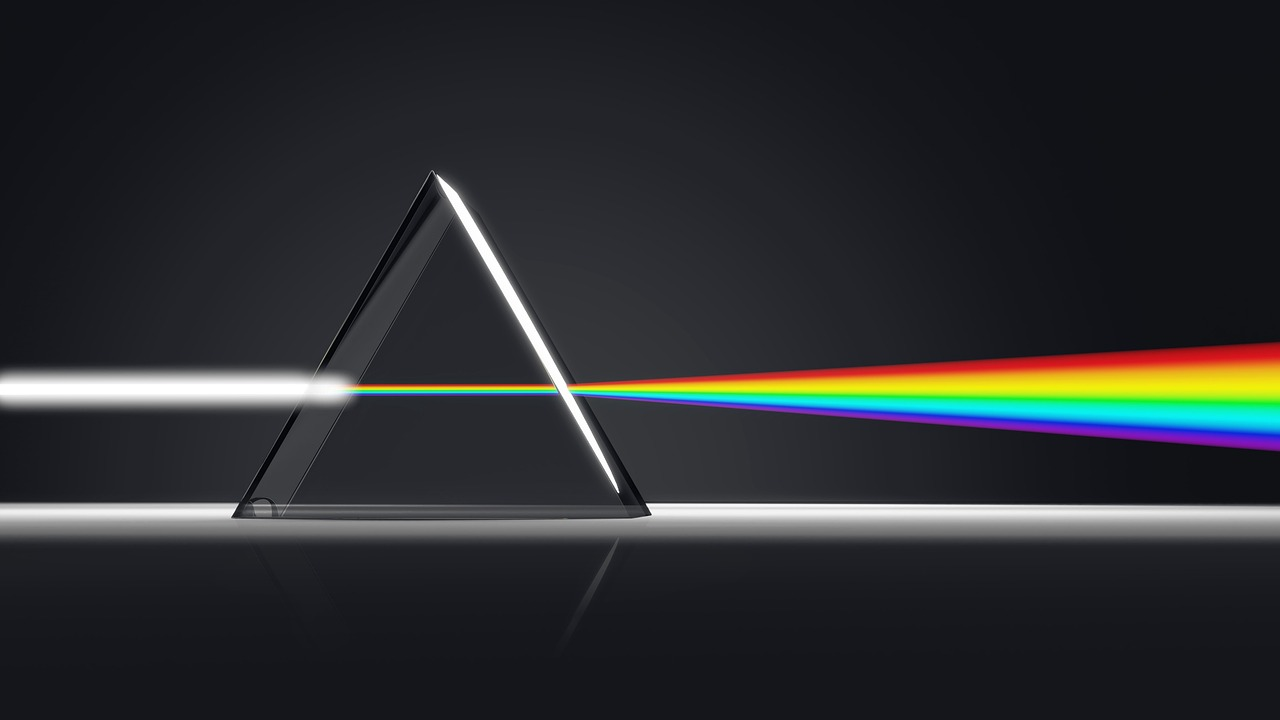
\includegraphics[width=6.5cm]{contents/images/prism-light-dispersion}
            };
        \end{tikzpicture}
    \end{frame}
}
\begin{frame}[fragile]{Feynman (3-Point Vertex)}
    \begin{columns}[onlytextwidth]
        \begin{column}{0.4\textwidth}
            \begin{center}
                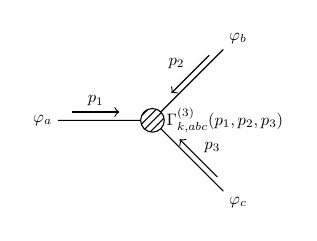
\begin{tikzpicture}[scale=0.6, every node/.style={transform shape}]
                    \draw (-2,0) node[left] {$\varphi_a$} -- (0,0) -- (1.5,1.5) node[above right] {$\varphi_b$} (0,0) -- (1.5,-1.5) node[below right] {$\varphi_c$};
                    \draw[->,yshift=5pt] (-1.7,0) -- (-0.7,0) node[midway,above] {$p_1$};
                    \draw[<-,yshift=5pt] (0.4,0.4) -- (1.2,1.2) node[midway,above left] {$p_2$};
                    \draw[<-,xshift=5pt] (0.4,-0.4) -- (1.2,-1.2) node[midway,above right] {$p_3$};
                    \draw[fill=white,postaction={pattern=north east lines}] (0,0) circle (0.25) node[right=5pt] {$\Gamma_{k,abc}^{(3)}(p_1,p_2,p_3)$};
                \end{tikzpicture}
            \end{center}
        \end{column}
        \begin{column}{0.5\textwidth}
            Beside, an example of tikz picture by \href{https://tikz.net/feynman-3/}{Janosh Riebesel l}. Below is a verbatim example, pay attention to the [fragile] parameter in line 123 (frame environtment).
        \end{column}
    \end{columns}
            \begin{block}{\tiny Feynman (3-Point Vertex)}
\begin{Verbatim}[fontsize=\tiny]
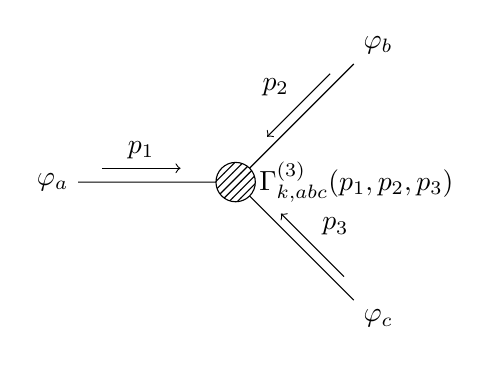
\begin{tikzpicture}
  \draw (-2,0) node[left] {$\varphi_a$} -- (0,0) -- (1.5,1.5) node[above right] {$\varphi_b$} (0,0) -- (1.5,-1.5) node[below right] {$\varphi_c$};
  \draw[->,yshift=5pt] (-1.7,0) -- (-0.7,0) node[midway,above] {$p_1$};
  \draw[<-,yshift=5pt] (0.4,0.4) -- (1.2,1.2) node[midway,above left] {$p_2$};
  \draw[<-,xshift=5pt] (0.4,-0.4) -- (1.2,-1.2) node[midway,above right] {$p_3$};
  \draw[fill=white,postaction={pattern=north east lines}] (0,0) circle (0.25) node[right=5pt] {$\Gamma_{k,abc}^{(3)}(p_1,p_2,p_3)$};
\end{tikzpicture}
\end{Verbatim}
            \end{block}
\end{frame}

\end{document}

%%% Local Variables:
%%% mode: latex
%%% TeX-master: t
%%% End:
